\documentclass{article}
\usepackage[utf8x]{inputenc}
\usepackage[english,hebrew]{babel}
\usepackage{amsmath} 
\selectlanguage{hebrew}
\usepackage[top=2cm,bottom=2cm,left=2.5cm,right=2cm]{geometry}
\usepackage{graphicx}
\graphicspath{ {./images/} }
\usepackage{wrapfig}
\usepackage{empheq}
\usepackage{dashbox}

\newcommand{\image}[2]{
    \begin{align*}
        \centering
        \includegraphics[scale=#2]{#1}
    \end{align*}
}

\title{נבחרת ישראל הצעירה בפיזיקה - מטלה 2 }
\author{איתי מור}
\begin{document}
\maketitle

\section*{שאלות פתוחות מהאימונים}
\subsection*{חוק הציפה של ארכימדס )שאלה פתוחה מהאימון של אשכול A(}
\begin{enumerate}
    \item 
    מסת הקובייה היא $a^3\rho$

    \item 
    קודם כל פועל על הקובייה כח כבידה בגודל: $a^3\rho g$.
    בנוסף, בגלל שהאוקיינוס שקט והמים בו לא זזים בכלל, שאר המים באוקיינוס חייבים להפעיל על הקוביה כח נגדי כלפי מעלה באותו גודל.
    \image{images/archimedes_rule_diagram1.png}{0.8}
    
    \item 
    ראשית, ברור שכח המשיכה יהיה שונה בהתאם לשונות המסה. כח המשיכה על הקובייה החדשה יהיה
    $Mg$.
    שנית, מכיוון שלמים יש אינטרקציה רק עם החלק החיצוני של הקובייה, הכח שהם מפעילים עליה יכול להיות תלוי רק בנפח הקוביה ולא יכול להשתנות בין צפיפויות שונות )המים לא יכולים להבדיל בין קוביית מים, לקוביית אחרת עם אותם מימדים(.
    כלומר כח הציפה יהיה זהה על שתי הקוביות ולכן גם על הקוביה המוצקה יפעל כח של:
    $a^3\rho g$.
    \image{images/archimedes_rule_diagram2.png}{0.64}

    \item 
    נסמן את צפיפות הקובייה המוצקה ב
    $\rho_2 = \frac{M}{a^3}$.
    התנאי שהקובייה תצוף אל פני המים הוא:
    \begin{flalign*}
        & Mg < a^3\rho g &&\\
        & a^3 \rho_2 < a^3 \rho &&\\
        & \rho_2 < \rho &&
    \end{flalign*}
    כלומר התנאי הוא שצפיפות הקובייה תהיה קטנה מצפיפות המים.


    \item 
    הקוביה מאיצה מעלה בתאוצה 
    $\frac{a^3\rho g - Mg}{M}$
    לכן המרחק שהיא תעבור אחרי $t$ שניות הוא:
    \begin{flalign*}
        & \frac{\left( \frac{a^3\rho g - Mg}{M} \right)t^2}{2} = H&&\\
        & t = \sqrt{\frac{2MH}{a^3\rho g - Mg}} &&
    \end{flalign*}
    מכיוון שאמרו שצלע הקובייה זניחה ביחס לגובה מתחת לפני המים שלה, אין צורך להתעסק בזמן שלוקח לפאות השונות שלה להגיע אל פני המים.

    \item 
    תחילה נחשב את המהירות של הקוביה רגע לפני שהיא יוצאת מהמים:
    \begin{flalign*}
        & v = \sqrt{\frac{2MH}{a^3\rho g - Mg}} \cdot \frac{a^3\rho g - Mg}{M} &&\\
        & v = \sqrt{\frac{2H\left(a^3\rho g - Mg\right)}{M}} && \\
    \end{flalign*}
    ברגע שהקובייה יוצאת מהים היא מתחילה להאיץ כלפי מטה בתאוצת הכובד.
    נחשב את פונקציית גובה הקוביה כתלות בזמן ונגזור כדי לקבל את הגובה המקסימלי:
    \begin{flalign*}
        & y(t) = t\sqrt{\frac{2H\left(a^3\rho g - Mg\right)}{M}} - \frac{gt^2}{2} &&\\
        & \frac{d\,y}{d\,t} = \sqrt{\frac{2H\left(a^3\rho g - Mg\right)}{M}} - gt = 0 &&\\
        & t = \sqrt{\frac{2H\left(a^3\rho - M\right)}{Mg}} &&\\
        & y_{max} = \sqrt{\frac{\left( 2H\left(a^3\rho - M\right) \right)^2}{M^2}} - \frac{H\left( a^3 \rho - M \right)}{M} &&\\
        & y_{max} = \frac{2H\left( 2H\left(a^3\rho - M\right) \right)}{M} - \frac{H\left( a^3 \rho - M \right)}{M} 
        = \frac{H\left( a^3 \rho - M \right)}{M} &&\\      
    \end{flalign*}

    \item 
    נתובנן בכוחות הפועלים על הקובייה.
    פועל עליה כח למטה $Mg$, ובנוסף פועל על החלק ששקוע בתוך המים של הקובייה כח ציפה כלפי מעלה.
    עם החלק התחתון של הקובייה היה מים, כח הציפה עליו היה 
    $a^2h\rho g$
    כדי לבטל את כח הכבידה עליו לכן זה גם אותו כח שיפעל הקובייה המוצקה.
    מהחוק הראשון של ניוטון נקבל:
    \begin{flalign*}
        & a^2h\rho g - Mg = 0 &&\\
        & M = a^2h \rho &&\\
        & h = \frac{M}{a^2\rho} &&
    \end{flalign*}
    \textbf{הערה:} במשוואה השנייה קיבלנו שאם החלק ששקוע במים של הקובייה היה מים, המסה שלו היתה מסת כל הקובייה.


    \item 
    כאשר כמות נפח בגודל של נפח החלק השקוע של קוביית הקרח יותך, מסת החלק הזה תהיה שווה למסת הקובייה כולה, )כפי שראינו בסעיף הקודם( כלומר עדיין הקובייה תפעיל את אותו הכח על המים ופני המים לא ישתנו. כעת יש חלק אחר של התיבה ששקוע במים וגם כאשר הוא יותך לא יקרה כלום וחוזר חלילה.
    כלומר פני המים לא יעלו ולא ירדו.
\end{enumerate}

\newpage
\subsection*{מעבר לכל ספיקה סבירה )שאלה פתוחה מהאימון של אשכול B(}
\begin{enumerate}
    \item
    חלקיק האבק ינוע במהירות הזרימה של הנוזל ולכן הוא יעבור מרחק 
    $ut$.

    \item 
    נפח הנוזל שחוצה חתך של הצינור הוא המרחק שחלקיק זורם בו לאורך פרק הזמן, כפול שטח החתך:
    \begin{flalign*}
        &V = Aut&&
    \end{flalign*}

    \item 
    ספיקת המסה היא הנפח שחישבנו בסעיף הקודם, כפול הצפיפות )כלומר מסת הנוזל שחצתה את חתך הצינור(, לחלק לפרק הזמן שלקח לנוזל לחצות את החתך:
    \begin{flalign*}
        & Q = \frac{\rho Aut}{t} = \rho Au &&
    \end{flalign*}
    \item 
    ספיקת המסה חייבת להיות זהה בשני קצוות הצינור מכיוון שבכל מקרה אחר בקצה מסויים כמות מסה כלשהי תנוע בקצב איטי יותר, ומסה תתחיל להצטבר בקצה זה עד שהצינור יכיל באיזור מסויים יותר מדי מים והוא יתפוצץ.
    לכן:
    \begin{flalign*}
        &Q_1 = Q_2&&
    \end{flalign*}

    \item 
    מכיוון שספיקת המסה נשארת זהה,
    מתקיים:
    \begin{flalign*}
        &\rho A_1 v_1 = \rho A_2 v_2&&\\
        &v_2 = \frac{A_1}{A_2} v_1&&
    \end{flalign*}

    \item 
    מכיוון שזה צינור רגיל שבו לשני הקצוות יש את אותו השטח, מהנוסחה מקבלים שמהירות המים בקצה העליון היא אותה מהירות שבה מזרימים את המים אל הקצה התחתון. כלומר המים יוצאים מהצינור במהירות $v$.
    \begin{flalign*}
        &y = (v\sin \alpha)t - \frac{gt^2}{2}&&\\
        &\dot{y} = v\sin\alpha - gt = 0&&\\
        &t = \frac{v\sin\alpha}{g}&&\\
        &y_{max} = \frac{v^2\sin^2\alpha}{g} - \frac{v^2\sin^2\alpha}{2g} = \frac{v^2\sin^2\alpha}{2g}&&
    \end{flalign*}

    \item 
    נסמן את שטח החתך בנק' הגבוהה ביותר של הזרנוק ב
    $A_2$.\\
    בנקודה הגבוהה ביותר של זרנוק המים, המהירות היא אופקית לחלוטין )כי השיפוע הוא 0(. בנקודה זו, מהירות הזרם היא 
    $v\cos\alpha$,
    לכן הספיקה של הזרם היא 
    $\rho A_2 v\cos\alpha$.
    מכיוון שהספיקה היא קבועה, הספיקה הזו שווה לספיקה שהיתה בתוך הצינור עצמו כלומר:
    \begin{flalign*}
        &\rho A_2 v\cos \alpha = \rho A v&&\\
        &A_2 = \frac{A}{\cos \alpha}&&
    \end{flalign*}
\end{enumerate}





\newpage
\section*{מכניקה}
\subsection*{שאלה מהתרגול}
נתבונן בכוחות הפועלים על החוליות בכל צד:
    \begin{align*}
        \centering
        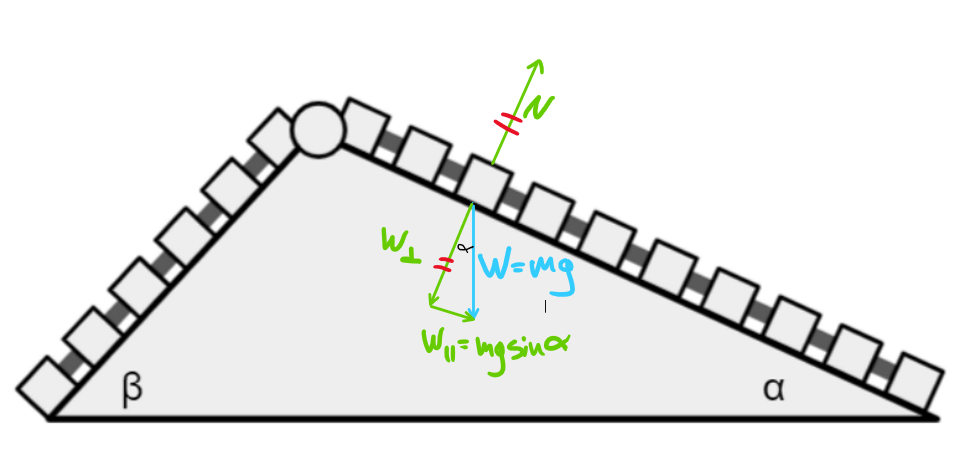
\includegraphics[scale=0.4]{images/from_tirgul_q5.png}
    \end{align*}
    
    \begin{align*}
        \centering
        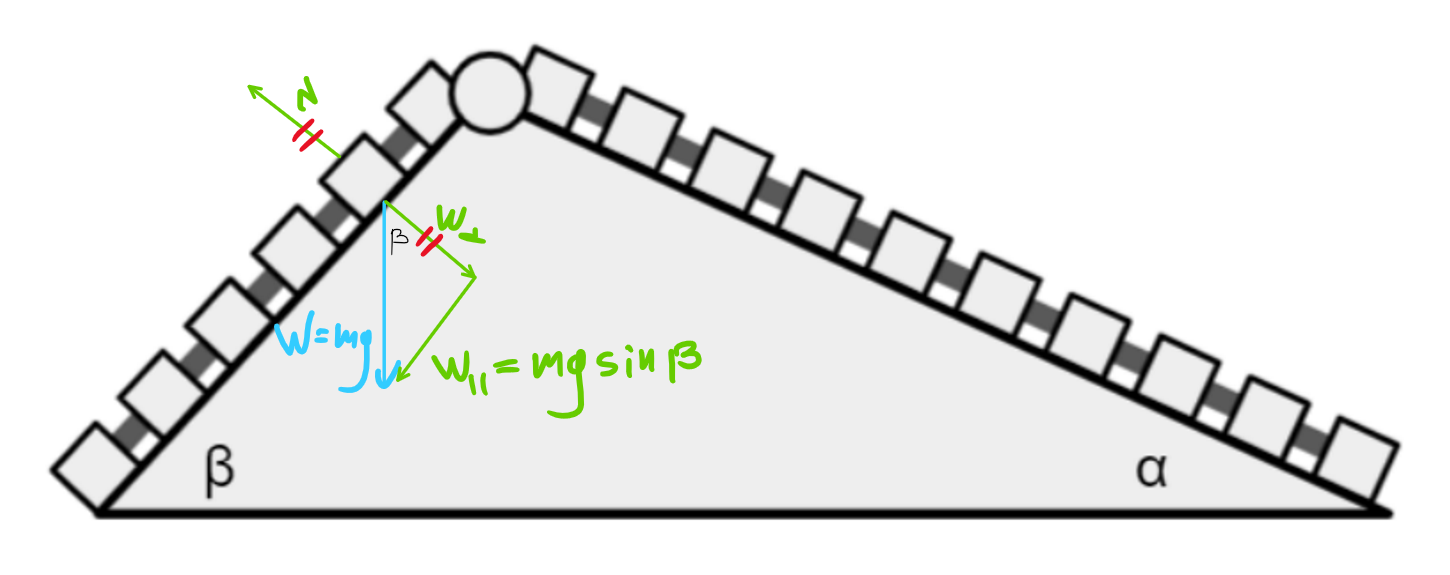
\includegraphics[scale=0.3]{images/from_tirgul_q5_b.png}
    \end{align*}
מכיוון שהכוחות המאונכים לטריז מבטלים אלו את אלו, הכוחות היחידים הפועלים על החוליות בשרשרת הם הכוחות הפועלים במקביל לטריז.\\
נסמן את אורך הצלע השמאלית של הטריז ב
$a$
ואת הצלע הימנית של הטריז ב
$b$.\\
ע"פ משפט הסינוסים:
\begin{equation*}
    \frac{a}{\sin \alpha} = \frac{b}{\sin \beta}
\end{equation*}
נכפיל את שני האגפים ב
$n$
ונקבל את כמות החוליות שיש בכל צד לחלק לסינוס הזווית שליד אותה הפאה של הטריז:
\begin{equation*}
    \frac{an}{\sin \alpha} = \frac{bn}{\sin \beta}
\end{equation*}
נסמן:
\begin{equation*}
    an\sin{\beta} = bn \sin{\alpha} = k
\end{equation*}
\\
נחשב את סכום הכוחות הפועלים על השרשרת )לצד שמאל(:
\begin{equation*}
    \Sigma{\vec{F}} = an \cdot mg\sin{\beta} - bn \cdot mg\sin{\alpha} = k(mg - mg) = 0
\end{equation*}
ולכן גם התאוצה היא $0$, כלומר השרשרת נעה במהירות קבועה )או במנוחה(.




\newpage
\subsection*{זינוק בירידה - המשך}
\begin{enumerate}
    \item 
    נפרק את תאוצת הכובד
    $g$
    לשני לרכיב מקביל למישור ורכיב מאונך למישור:
    $g_{\parallel}, g_{\perp}$.\\
    \begin{flalign*}
        &g_{\perp} = g\cos{\alpha}&&\\
        &g_{\parallel} = g\sin{\alpha}&&\\
    \end{flalign*}
    \begin{align*}
        \centering
        \fbox{
            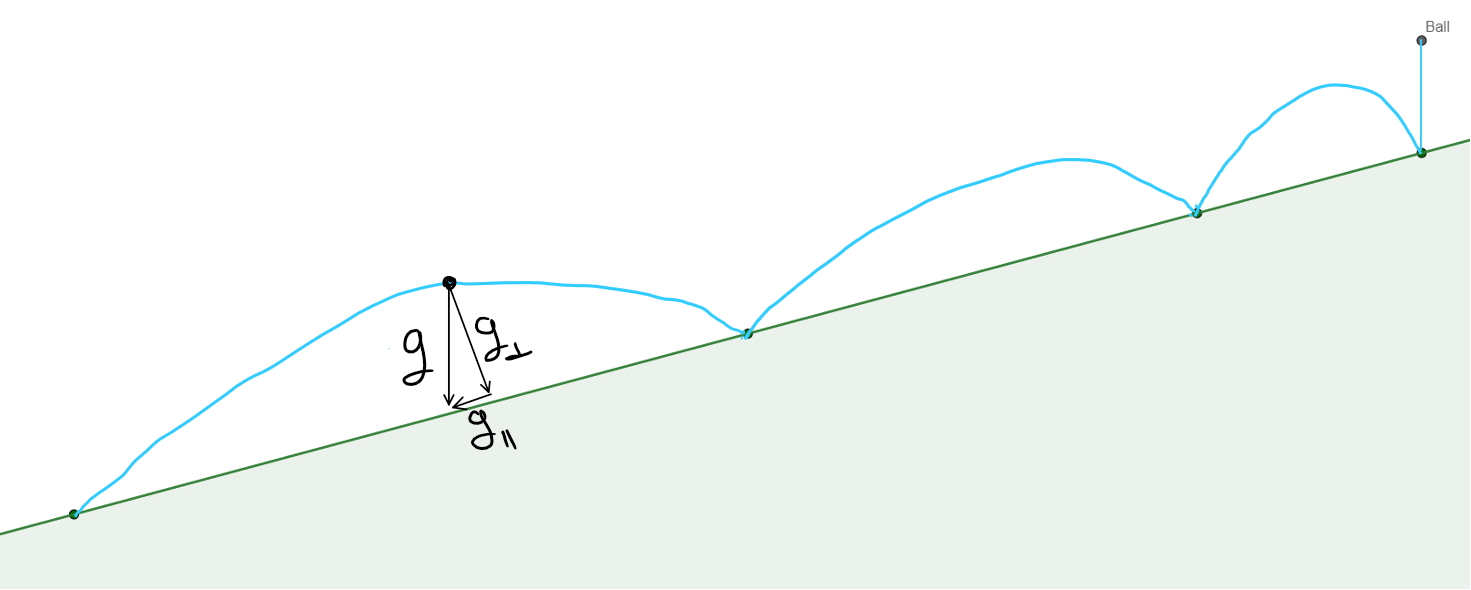
\includegraphics[scale=0.4]{images/jump_on_lowering_diagram1.png}
        }
    \end{align*}
    בחלק הראשון של השאלה הזאת )במטלה הקודמת( ראינו שמהירות הפגיעה הראשונה הכוללת היא 
    $\sqrt{2gh}$
    כלומר המהירות המאונכת )למישור( היא 
    $\sqrt{2gh}\cos{\alpha}$.\\
    מכיוון שבציר המאונך הכדור נופל כל הזמן נפילות חופשיות )בתאוצה 
    $g_{\perp}$(
    המהירות האנכית בתחילת כל קפיצה שווה למהירות האנכית בסוף כל קפיצה. כלומר בין קפיצות, גודלה של המהירות האנכית נשמר )ומשנה כיוון(.
    לכן משך כל הקפיצות זהה.
    נחשב את משך הקפיצה:
    \begin{flalign*}
        &r_{\perp}(\Delta t) = \sqrt{2gh}\;\Delta t\cos{\alpha} - \frac{g_{\perp}{\Delta t}^2}{2} = 0&&\\
        &\sqrt{2gh}\;\Delta t\cos{\alpha} = \frac{g\cos{\alpha}\;{\Delta t}^2}{2}&&\\
        &\Delta t = \sqrt{\frac{8h}{g}}&&
    \end{flalign*}
    לכן זמן הפגיעה ה
    $n$-ית
    הוא 
    $n$ 
    פעמים משך הקפיצה הזו ועוד הזמן שלוקח עד שהכדור פוגע במישור בפעם הראשונה:
    \begin{flalign*}
        &t_n = n\Delta t + \sqrt{\frac{2h}{g}}&&\\
        &t_n = (2n - 1)\sqrt{\frac{2h}{g}}&&\\
    \end{flalign*}

    \item 
    כעת נפתור את הבעיה באמצעות הסתכלות עליה בציר המקביל למישור.\\
    מכיוון שהפגיעות במישור מפעילות כח נורמלי רק בכיוון המאונך למישור, התאוצה בכיוון המקביל למישור קבועה ולכן:
    \begin{flalign*}
        &D_\parallel(t_n) = \frac{g_\parallel \; {t_n}^2}{2}&&\\
        &D_\parallel(t_n) = \frac{g\sin{\alpha} \; (2n-1)^2\left(\frac{2h}{g}\right)}{2}&&\\
        &D_\parallel(t_n) = h(2n-1)^2\sin{\alpha}&&\\
        &x_n = D_\parallel(t_n)\cos\alpha = h(2n-1)^2\sin{\alpha}\cos{\alpha} = \frac{h}{2} (2n-1)^2 \sin{(2\alpha)}&&\
    \end{flalign*}
    אבל צריך לזכור לחסר את המרחק בציר ה $x$ שהכדור ככיבול עובר עד הפגיעה הראשונה מכיוון שהמיקום האופקי של הפגיעה הראשונה הוא 0:
    \begin{align*}
    \centering
        \fbox{
            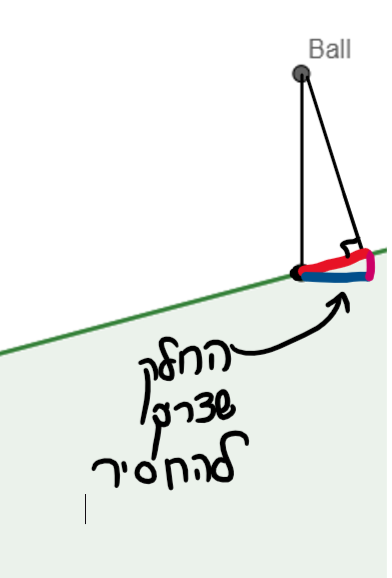
\includegraphics[scale=0.4]{images/jump_on_lowering_diagram2.png}
        }
    \end{align*}
    \begin{flalign*}
        &x_n = \frac{h}{2} (2n-1)^2 \sin{(2\alpha)} - \frac{h}{2} (2-1)^2 \sin{(2\alpha)} =  2nh(n-1) \sin{(2\alpha)}
    \end{flalign*}
\end{enumerate}




\newpage
\subsection*{הרמת משקולות}
\image{images/t2_q2_diagram.png}{0.4}
\begin{enumerate}
    \item 
    מהשרטוט ניתן לראות שמופעל על הפלטפורמה התחתונה כח של 
    $4T$
    )ארבעה קצוות חבל שנכנסים ויוצאים מהגלגלת התחתונה(.\\
    בנוסף, מהחוק השלישי של ניוטון בגלל שאלה מושכת את החבל למטה בכח 
    $T$,
    החבל מפעיל על אלה כח 
    $T$
    למעלה, כלומר היא לא מפעילה את כל כח הכבידה שלה על הפלטפורמה.
    מהחוק הראשון של ניוטון נקבל
    \begin{flalign*}
        &4T = Mg + mg - T&&\\
        &5T = (m+M)g&&\\
        &T = (m+M)\frac{g}{5}&&
    \end{flalign*}
    לכן אלה צריכה למשוך את החבל בכח 
    $T = \frac{\displaystyle (m+M)g}{\displaystyle 5}$.

    \item 
    מכיוון שקצה החבל שאלה משכה, "התארך" ב
    $D$,
    כל חלקי החבל במערכת הגלגלות משמאל לאלה, צריכים ביחד "להתקצר" ב
    $D$.
    מכיוון שהמתיחות חייבת להשמר לאורך החבל, כל קצוות החבל חייבים להתקצר באותו אורך )אחרת חלק מהקצוות יהיו "משוחררים"(
    לכן כל קצה חבל יתקצר ב
    $\frac{D}{4}$
    וזה יהיה הגובה בו אלה והבלוק יעלו ביחס לקרקע.
\end{enumerate}

\newpage
\subsection*{גלגל הגלגלות}
\image{images/wheels_wheel.png}{0.4}
\begin{flalign*}
    &L=2\sum_{j\;=\;1}^{n} l_j \qquad\qquad\qquad \Bigg/\frac{d^2}{d^2 t}&&\\
    &0=\ddot{L}=2\sum_{j\;=\;1}^{n} a_j \quad\quad\quad\quad \Bigg/ :2 &&\\
    &\sum_{j\;=\;1}^{n} a_j = 0&&
\end{flalign*}

נשתמש בחוק השני של ניוטון על מסה 
$m_i$
כלשהי:\\
\begin{flalign*}
    &m_i a_i = 2T-m_i g \qquad\qquad\qquad \Bigg/ : m_i &&\\
    &a_i = \frac{2T}{m_i} - g &&
\end{flalign*}

כעת נסכום את המשוואות עבור כל המסות:
\begin{flalign*}
    & 2T \left( \sum_{j\;=\;1}^{n} \frac{1}{m_j} \right) - n g = \sum_{j\;=\;1}^{n} a_j = 0 &&\\
    & 2T = g \frac{n}{\displaystyle \sum_{j\;=\;1}^{n} \frac{1}{m_j}} = g \cdot H(m_1, m_2, \dots, m_n) &&
\end{flalign*}
נציב את המתיחות שמצאנו בנוסחה לתאוצה של גוף כללי:
\begin{flalign*}
    & a_i = \frac{g}{m_i} H(m_1, m_2, \dots, m_n)\;-\;g &&
\end{flalign*}
\textbf{הערה: }
$H(m_1, m_2, \dots, m_n)$
זה הממוצע ההרמוני של המסות.



\newpage
\section*{חשבון דיפרנציאלי}
\subsection*{כללי נגזרות}
\begin{enumerate}
  \item \textbf{כלל המכפלה:} \\
    נפרק את מכפלת הפונקציות כמתואר באיור הבא: 
    \image{images/derivative_drawing.png}{0.4}
    
    \begin{flalign*}
      \frac{d (f g)}{d x} = \lim_{h \to 0}{\frac{f(x+h)g(x+h) - f(x)g(x)}{h}} 
      = \lim_{h \to 0}{ \frac{ g(x+h) \cdot \left[ f(x+h)-f(x) \right] + f(x) \cdot \left[ g(x+h) - g(x) \right]}{h} } &&
    \end{flalign*}
    \begin{flalign*}
        = \frac{d f}{d x} \cdot \lim_{h \to 0}{g(x+h)}  + \frac{d g}{d x} \cdot \lim_{h \to 0}{f(x)} 
        = \frac{d f}{d x} g + \frac{d g}{d x} f&&
    \end{flalign*}

  \item \textbf{כלל המנה:}
    \begin{flalign*}
        \frac{d \left( \frac{f}{g}\right)}{d x} = \lim_{h \to 0}{\frac{\frac{f(x+h)}{g(x+h)} - \frac{f(x)}{g(x)}}{h}}
        = \lim_{h \to 0}{\frac{\frac{f(x+h)g(x) - f(x)g(x+h)}{g(x)g(x+h)}}{h}}
        = \frac{\displaystyle \lim_{h \to 0}{\frac{f(x+h)g(x)-g(x+h)f(x)}{h}}}{\displaystyle \lim_{h \to 0}{g(x)g(x+h)}}&&
    \end{flalign*}
    \begin{flalign*}
        = \frac{\displaystyle \lim_{h \to 0}{\frac{f(x+h)g(x) - g(x+h)f(x) + g(x)f(x) - g(x)f(x)}{h}}}{g^2(x)}&&
    \end{flalign*}
    \begin{flalign*}
        = \frac{\displaystyle \lim_{h \to 0}{g(x) \cdot [f(x+h) - f(x)]} - \lim_{h \to 0}{f(x) \cdot [g(x+h) - g(x)]}}{g^2(x)}
        = \frac{f(x) \frac{d f}{d x} - g(x) \frac{d g}{d x}}{g^2(x)}&&
    \end{flalign*}
  \item \textbf{כלל השרשרת:}\\
    נשתמש בהגדרה השנייה של נגזרת:
    \begin{flalign*}
        &\frac{d\,f(g(x))}{d\,x}=\lim_{x \to x_0}{\frac{f(g(x_0)) - f(g(x))}{x_0 - x}}&&
    \end{flalign*}
    נרחיב את המונה והמכנה ב 
    $g(x_0) - g(x)$:
    \begin{flalign*}
        &\lim_{x \to x_0}{\frac{[f(g(x_0)) - f(g(x))]\cdot[g(x_0) - g(x)]}{[g(x_0) - g(x)]\cdot[x_0 - x]}}&&\\
        &\lim_{x \to x_0}{\frac{f(g(x_0)) - f(g(x))}{g(x_0) - g(x)}} \cdot \lim_{x \to x_0}{\frac{g(x_0) - g(x)}{x_0 - x}}&&
    \end{flalign*}
    מכיוון ש
    $g$
    גזירה בסביבות הנקודה
    $x_0$,
    היא בהכרח גם רציפה בסביבה זו. כלומר הביטוי
    $x \to x_0$,
    שקול ל-
    $g(x) \to g(x_0)$
    לכן הגבול מלמעלה שקול לגבול:
    \begin{flalign*}
        &\lim_{g(x) \to g(x_0)}{\frac{f(g(x_0)) - f(g(x))}{g(x_0) - g(x)}} \,\cdot \lim_{x \to x_0}{\frac{g(x_0) - g(x)}{x_0 - x}} =
        \frac{d\,f}{d\,g}\cdot\frac{d\,g}{d\,x}&&
    \end{flalign*}
\end{enumerate}





\newpage
\subsection*{מן הפח אל הפחית}
\begin{enumerate}
  \item הכוונה בעובי קטן מאוד היא עובי קטן מאוד ביחס לרדיוס הפחית ולגובה הפחית כדי שהעובי לא ישפיע על נפח הפחית:
  \begin{align*}
      width \ll r \\
      width \ll h
  \end{align*}
    



  \item קל לראות שעלות הייצור של פחית תלוייה ישירות בשטח הפנים שלה )מכיוון ששטח הפנים כפול עובי הפחית כפול עלות פח נותן את עלות הייצור( .\\
  נפח הפחית הוא $V = \pi h r^2$,
  כלומר:

  \begin{equation*}
      h = \frac{V}{\pi r^2}
  \end{equation*}

  שטח הפנים של הפחית כתלות ברדיוס הוא: 
  \begin{equation*}
      A(r) =  2\pi r\left( h+r \right) = 2\pi hr + 2\pi r^2
  \end{equation*}
  נציב את הערך של הגובה שקיבלנו:
    \begin{equation*}
      A(r) =  2\pi r \cdot \frac{V}{\pi r^2} + 2\pi r^2 = \frac{2V}{r} +2\pi r^2
    \end{equation*}
  נגזור את הפונקציה ונשווה ל-0 כדי לקבל את שטח הפנים המינימאלי שיוצר נפח $V$:

  \begin{equation*}
    A'(h) = -\frac{2V}{r^2} + 4\pi r = 0
  \end{equation*}
  \begin{equation*}
      r^3 = \frac{V}{2\pi}
  \end{equation*}
  \begin{equation*}
      r = \sqrt[\leftroot{-2}\uproot{2}3]{\frac{V}{2\pi}}
  \end{equation*}
    \begin{equation*}
      V = h\pi r^2
  \end{equation*}
  \begin{equation*}
      V = h\pi\sqrt[\leftroot{-2}\uproot{2}3]{\frac{V^2}{4\pi^2}} = h\sqrt[\leftroot{-2}\uproot{2}3]{\frac{V^2\pi}{4}}
  \end{equation*}
    \begin{equation*}
        h = \frac{V}{\sqrt[\leftroot{-2}\uproot{2}3]{\frac{V^2\pi}{4}}}
        = \sqrt[\leftroot{-2}\uproot{2}3]{\frac{V^3}{\frac{V^2\pi}{4}}}
        = \sqrt[\leftroot{-2}\uproot{2}3]{\frac{4V}{\pi}}
    \end{equation*}

    \begin{equation*}
        \frac{r}{h} =\sqrt[\leftroot{-2}\uproot{2}3]{\frac{\frac{V}{2\pi}}{\frac{4V}{\pi}}} = \sqrt[\leftroot{-2}\uproot{2}3]{\frac{1}{8}} = \frac{1}{2}
    \end{equation*}
    כלומר היחס בין הרדיוס לגובה שנותן את העלות המינימלית הוא $1 : 2$

    \item בפחית קוקה קולה רגילה,היחס בין הרדיוס לגובה הוא $\frac{6}{31}$:
    \image{images/can_measures.png}{0.4}
    נסמן את פונקצית עלות הייצור של הפחית כתלות ברדיוס ב
    $f(r)$,
    את עובי הבסיסים ב
    $w_b$
    ואת עובי המעטפת ב
    $w_s$.
    \begin{flalign*}
        f(r)=2\pi r^2 w_b + 2\pi r h w_s&&
    \end{flalign*}
    מנוסחאת נפח של פחית נקבל-
    \begin{flalign*}
        &V = \pi r^2 h&&
        \\&h = \frac{V}{\pi r^2}&&
    \end{flalign*}
    נציב בפונקציית עלות הייצור ונקבל:
    \begin{flalign*}
        &f(r) = 2\pi r^2 w_b + \frac{2\pi r V w_s}{\pi r^2} = 2\pi r^2 w_b +\frac{2V}{r}w_S&&
    \end{flalign*}
    נגזור את הפונקציה ונשווה ל-0 כדי למצוא נקודת קיצון:
    \begin{flalign*}
        &\frac{d\,f}{d\,r} = 4\pi r w_b - \frac{2V}{r^2} w_s = 0&&
      \\&4\pi r w_b = \frac{2V}{r^2}w_s&&
      \\&\frac{2\pi r^3}{V} = \frac{w_s}{w_b}&&
      \\&\frac{2\pi r^3}{\pi r^2 h} = \frac{w_s}{w_b}&&
      \\&\frac{2r}{h} = \frac{w_s}{w_b}&
      \\&\frac{w_s}{w_b} = \frac{12}{31} \approx \frac{2}{5}
    \end{flalign*}
    זוהי בהכרח נק' מינימום מכיוון שגם כשהיחס בין הרדיוס לגובה שואף לאינסוף )הרדיוס שואף לאינסוף והגובה שואף לאפס( עלות הייצור שואפת לאינסוף וגם כשהיחס בין הרדיוס לגובה שואף לאפס )הגובה שואף לאינסוף והרדיוס שואף לאפס( עלות הייצור שואפת לאינסוף:
    \begin{flalign*}
        \lim_{r \to \infty}{2\pi r(\frac{V}{2\pi r}+r)} = \infty&&
    \end{flalign*}
    \begin{flalign*}
        \lim_{r \to 0^+}{2\pi r(\frac{V}{\pi r^2}+r)} = 2\pi\lim_{r \to 0}{r^2 + \frac{V}{\pi r}} = 2\pi(0 +\infty) = \infty&&
    \end{flalign*}
\end{enumerate}





\newpage
\subsection*{באש...}
אם נשקף את האש ביחס לים, נוכל למתוח קטע בין שגיא לשיקוף, וזה יהיה המרחק הקצר ביותר בין השיקוף לשגיא.\\
מכיוון שקו המים הוא אנך אמצעי לקטע שבין האש לשיקוף, המרחקים מנק' החיתוך של הקטע שמתחנו מקודם, לאש ולשיקוף של האש, שווים:
\image{images/geogebra-export.png}{0.4}
לכן אותה נק' חיתוך היא בהכרך הנקודה שממנה שגיא לוקח מים.
\image{images/on_fire_figure_with_angles.png}{0.4}
זווית $\alpha$ שווה ל-$\frac{\pi - \theta}{2}$.\\
נסמן את המרחק על ציר ה
$y$ 
בין נק' לקיחת המים לאש ב
$y_1$,
ואת המרחק על ציר ה
$y$
בין נק' לקיחת המים לשגיא ב
$y_2$.\\
בנוסף נסמן את המרחק הכולל ב
$y_1+y_2 = h$
\begin{equation*}
    \tan (\alpha) = \frac{y_1}{d_1}
\end{equation*}
\begin{equation*}
    \tan (\alpha) = \frac{y_2}{d_2}
\end{equation*}
\\
\\
\begin{equation*}
    y_1 + y_2 = (d_1 + d_2)\tan (\alpha) 
\end{equation*}
\begin{equation*}
    \frac{h}{d_1 + d_2} = \tan (\alpha) 
\end{equation*}
\begin{equation*}
    \alpha = \tan ^ {-1} \left( \frac{h}{d_1 + d_2} \right)
\end{equation*}
\begin{equation*}
    \frac{\pi}{2} - \frac{\theta}{2} = \tan ^ {-1}\left( \frac{h}{d_1 + d_2} \right)
\end{equation*}
\begin{equation*}
    \theta = \pi - 2\tan ^ {-1} \left( \frac{h}{d_1 + d_2} \right)
\end{equation*}


\newpage
\subsection*{ובמים...}
נניח שקיים מסלול A בין שגיא לילד הטובע.
כעת נסתכל על מסלול B, שחותך את קו החוף במרחק 
$dy$
ששואף לאפס ממסלול A.\\
מכיוון שהמרחק על קו החוף בין המסלולים שואף לאפס, גם הזוויות בין המסלולים ישאפו לאפס:
\image{images/and_in_the_water_diagram.png}{0.8}
לכן הקטע הצהוב זה הקטע שמתווסף למסלול, והקטע הטורקיז זה הקטע שיורד מהמסלול.\\
נרצה לחשב את השינוי בזמן שלוקח לשגיא להגיע לילד ביחס לשינוי ב
$dy$.
הזמן שמתווסף הוא 
$u\cdot dy\cos \beta$,
והזמן שיורד הוא
$v\cdot dy\cos \alpha$.\\
לכן:
\begin{flalign*}
    &dT=dy(u\cos{\beta} - v\cos{\alpha})&&\\
    &\frac{dT}{dy} = u\cos{\beta} - v\cos{\alpha}&&
\end{flalign*}
אנחנו מחפשים את נקודת המינימום, כלומר נקודה שבה כש $dy$ שואף לאפס
גם $dT$ שואף לאפס.
\begin{flalign*}
    &\frac{dT}{dy} = u\cos{\beta} - v\cos{\alpha} = 0&&\\
    &u\cos{\beta} = v\cos{\alpha}&&
\end{flalign*}

בנוסף, קיים עוד קשר בין שתי הזוויות:
\image{images/CamScanner 10-05-2023 20.48.jpg}{0.1}
כלומר:
\begin{flalign*}
    &d_1 \cot \alpha + d_2 \cot \beta = D&&
\end{flalign*}

כלומר התנאים על הזוויות הם:
\begin{empheq}[left=\empheqlbrace]{equation*}
    \begin{flalign*}
        &u\cos{\beta} = v\cos{\alpha}&&\\
        &d_1 \cot \alpha + d_2 \cot \beta = D&&
    \end{flalign*}
\end{empheq}




\end{document}